\chapter{Práctica Mónaco}
\label{ch:PracticaMonaco}

Una vez explicado el contexto, los objetivos y las herramientas usadas en el proyecto, en este capítulo vamos ver en detalle la construcción de un mundo para JdeRobot, en concreto el circuito de Fórmula 1 de Mónaco.


\section{Manejo de Blender}
\label{sec:pm_manejodeblender}

En esta sección vamos a explicar cómo se utiliza este potente programa de creación, renderizado y animación de gráficos tridimensionales. El uso de este tipo de programas es, a priori, de los más difíciles, ya que trabajar sobre un mundo tridimensional en una pantalla de ordenador, desplazando un ratón sobre una mesa en dos dimensiones, exige un esfuerzo de abstracción considerable.


Es por ello que en los primeros pasos de esta sección nos dedicaremos a presentar la interfaz del programa y exponer la inmensa cantidad de opciones y herramientas de que dispone, centrándonos en aquellas que han resultado relevantes para la consecución de los objetivos marcados.


\subsection{Interfaz}
\label{subsec:pm_interfaz}

Como se verá, la interfaz de Blender no sigue el patrón típico de los programas a los que estamos habituados, como editores de texto y hojas de cálculo o entornos de desarrollo de software, por lo que resulta fácil desorientarse al principio.

La interfaz de usuario de Blender está compuesta por 4 ventanas por defecto como se pueden diferenciar en la imagen (\textit{Figura \ref{fig:interfazblender01}}). Cada ventana tiene una cabecera con las herramientas adecuadas para trabajar sobre
dicha ventana y, a su vez, cada herramienta está dotada de sus correspondientes pestañas para una completa edición. Esta disposición facilita y agiliza el uso apropiado del programa. A su vez, cada cabecera de cada ventana tiene el botón Tipo de Editor, mediante el cual se puede cambiar el tipo de ventana que se muestra, por lo que se puede personalizar el aspecto para agilizar el trabajo.

\begin{figure}[ht]
	\centering
	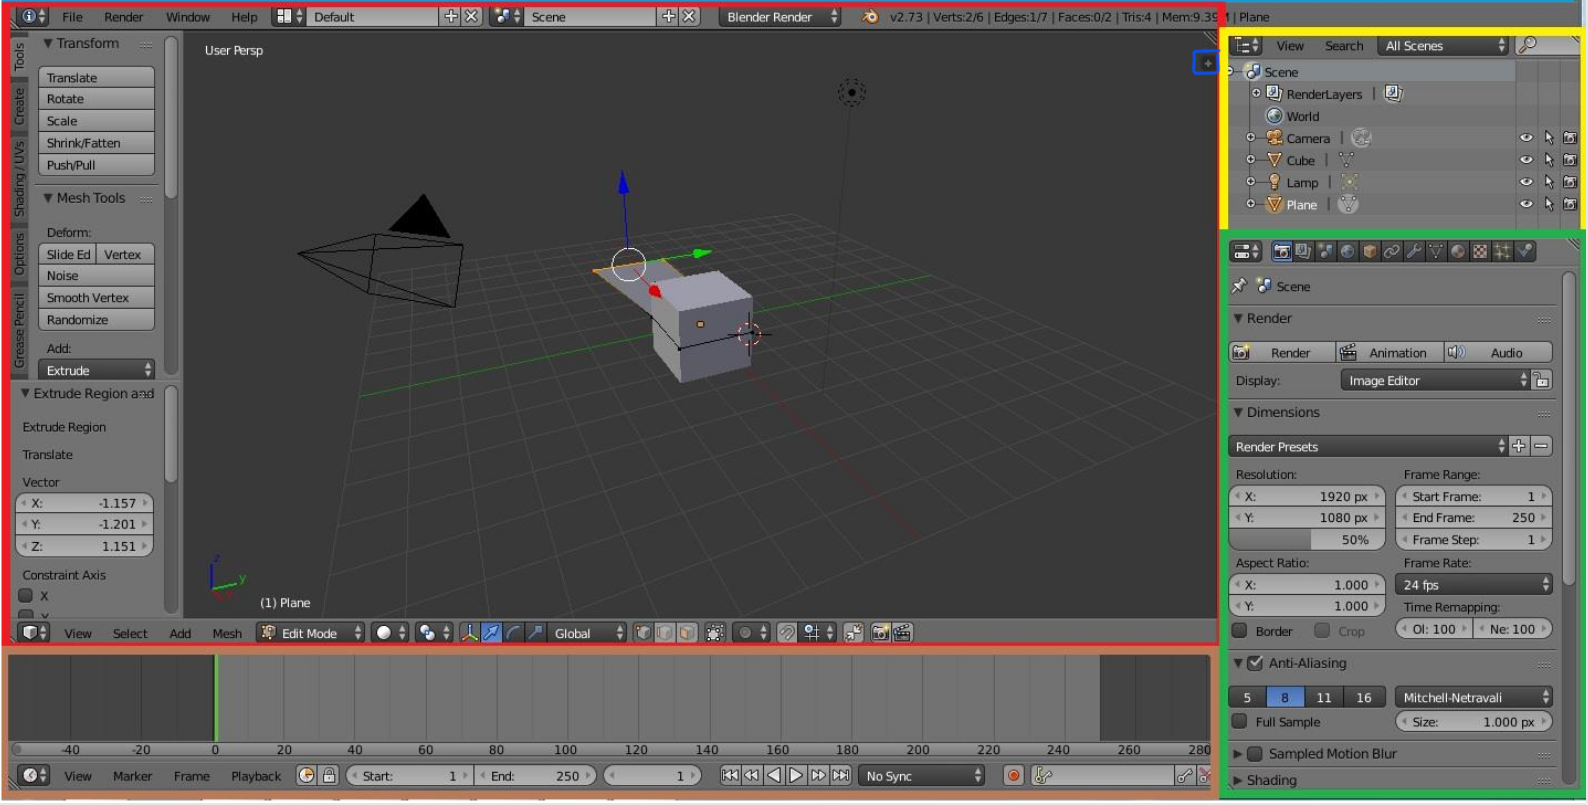
\includegraphics[width=0.9\textwidth]{InterfazBlender01.png}
	\caption{Interfaz de Blender.} \label{fig:interfazblender01}
\end{figure}


En primer lugar tenemos la ventana de Vista 3D, bordeada en color Rojo. En esta ventana se visualiza todo el trabajo y los cambios que se realizan con el programa.

En esta ventana podemos observar los siguientes objetos y menús:

\begin{itemize}
	\item Manipuladores de Transformaciones en 3D (\textit{Figura \ref{fig:interfazblender03}}): Muestra de manera visual información de las transformaciones a realizar. Cada objeto puede ser transformado de tres maneras: traslación (G), rotación (R) y escalado (S). Utilizando la combinación Ctrl+Space,	o bien haciendo clic en el icono del sistema de coordenadas, se puede mostrar y ocultar el manipulador. 
	\begin{figure}[h]
		\centering
		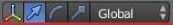
\includegraphics[width=0.25\textwidth]{InterfazBlender03.png}
		\caption{Detalle de Manipuladores de transformaciones en 3D.} \label{fig:interfazblender03}
	\end{figure}
	
	
	\item Cursor 3D (\textit{Figura \ref{fig:interfazblender04}}): El cursor 3D es una herramienta muy útil y se utiliza para una variedad de cosas como representar el lugar donde se añadirán nuevos objetos o representar el punto de pivote para una rotación. Sin embargo es muy engorroso a la hora de trabajar ya que es muy fácil moverlo accidentalmente y al necesitar usarlo se pierde bastante tiempo reubicándolo.
	\begin{figure}[h]
		\centering
		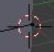
\includegraphics[width=0.05\textwidth]{InterfazBlender04.png}
		\caption{Detalle del cursor de Blender.} \label{fig:interfazblender04}
	\end{figure}

	\item Cubo: Al iniciar Blender, por defecto, aparece un cubo situado en el centro de la ventana 3D. Es uno de los elementos básicos que se pueden insertar y la mayoría de las veces basta con este simple cubo para comenzar a trabajar.
	
	\item Luz (de tipo lámpara): Al iniciar Blender, por defecto, también aparecerá una Luz de tipo lámpara que estará en algún sitio cerca del centro de la escena. Es posible crear otras fuentes de luz, como un sol en el cenit de la escena o una luz direccional que ilumine todos los objetos. En cualquier caso, aunque en los diferentes modos de edición no sea necesario, a la hora de renderizar la escena para visualizar el resultado del trabajo es necesaria alguna fuente de luz, si no aparecerá una escena llena de siluetas.
	
	\item Cámara: Al iniciar Blender, por defecto, aparecerá una cámara que estará en algún sitio por el centro de la ventana 3D y, probablemente, enfocando al cubo. En la figura \ref{fig:interfazblender01} es esa especie de pirámide de vértices negros a la izquierda del cubo. A la hora de renderizar es necesaria una cámara.
	
	\item Objeto seleccionado actualmente: Este campo, situado en la parte inferior izquierda de la escena, al lado del eje de coordenadas, muestra el  nombre del objeto seleccionado actualmente.
	
	\item Modo Edición: Este botón, en forma de desplegable, se encuentra a la izquierda de los botones de manipuladores de transformaciones 3D. Da acceso a un modo de edición para manipular la geometría del objeto. Al activarse aparecen disponibles tres botones de opciones, justo a la derecha de los botones de manipuladores de transformaciones 3D. Nos permiten cambiar entre la selección y edificación de los vértices, de las aristas y de las caras del objeto. la posibilidad de cambiar entre estas opciones de selección se presta especialmente útil a la hora de dar forma a los objetos que componen el circuito.
	
	\item Vista de la escena: Este botón, en forma de desplegable, se encuentra a la derecha del botón de Modo Edición. Da acceso a un desplegable que permite elegir la vista de la escena 3D entre las posibles, como sólida, texturas, materiales, ”wireframe”, renderizada, etc. Nos permite ver los objetos de la escena con sólo las texturas, sólo los vértices, ya renderizado, etc, para poder trabajar más cómodo en según que condiciones y ver los resultados de aplicar texturas o del renderizado final.
	
\end{itemize}

Para poder realizar con comodidad el trabajo sobre cualquier tipo de elemento existen diferentes vistas disponibles, cada una con un atajo de teclado propio, en concreto del teclado numérico. De esta forma para el ”1” el programa proporcionara una vista frontal de la escena; con el número “3” se obtiene una vista derecha; etc... Una de las más cómodas para realizar el trabajo es la que le corresponde al número “7” ya que se trata de una vista cenital, que una vez superpuesto el plano del circuito facilitan la tarea de trazar el recorrido. Por último con la tecla “5” podemos cambiar la vista de Perspectiva a Ortográfica. La vista Perspectiva es la más similar a la realidad, dando profundidad a la escena y sensación de lejanía y proximidad de los objetos. La vista Ortográfica es más artificial, pues es como una proyección de la anterior, pero es útil en determinadas situaciones para no alterar las proporciones o manejar con fluidez objetos que quedarían tapados de otra forma.

Ésta ventana posee un botón de propiedades propio marcado en color Azul en la parte superior derecha, el cual despliega la ventana de propiedades (\textit{Figura \ref{fig:interfazblender02}}). Esta ventana muestra las propiedades del objeto seleccionado y resulta muy útil a la hora de añadir nuevos bloques o realizar modificaciones de los ya existentes, pudiendo modificar la localización, rotación, escala, etc...

\begin{figure}[h]
	\centering
	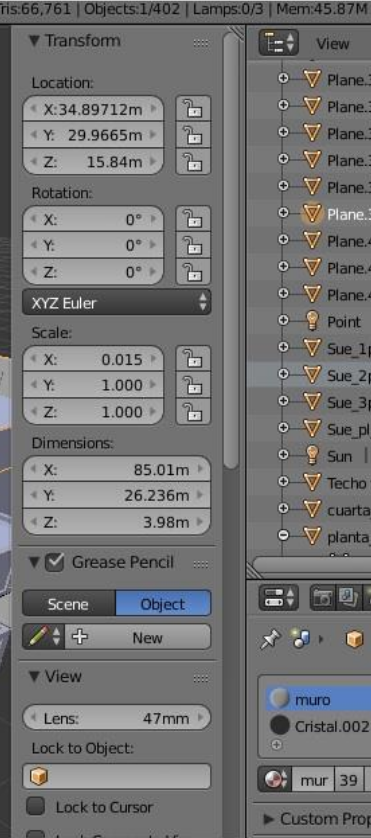
\includegraphics[width=0.2\textwidth]{InterfazBlender02.png}
	\caption{Ventana de propiedades.} \label{fig:interfazblender02}
\end{figure}

Debajo de la ventana de vista 3D, bordeada en Marrón, se encuentra por defecto la ventana de Línea Temporal. Aquí se reflejan cronológicamente los bloques u objetos que se han añadido o modificado y es muy utilizada al trabajar con animaciones. En nuestro caso la hemos sustituido por otra que se adapta mejor a nuestras necesidades.

A continuación, bordeada en Amarillo, se puede identificar la ventana de Objetos y Jerarquías, donde se pueden ver todos los datos que se utilizan en el trabajo. De esta forma se pueden controlar los diferentes bloques que se utilicen, las luces que se añaden a la escena, cámaras y toda clase de elementos disponibles en la escena. En esta ventana se pueden seleccionar directamente los elementos que se deseen independientemente, y realizar acciones sobre ellos como restringir o habilitar la visualización, selección o renderización de dicho elemento. Esto supone una gran ayuda cuando se superponen diferentes elementos en la ventana.

Debajo de ésta, marcada en color Verde, se encuentra la ventana de Propiedades, en la cual se pueden editar las propiedades de los bloques, objetos, materiales, texturas etc... que se utilizan en el trabajo. Esto se consigue mediante los llamados botones de contexto, los cuales muestran un grupo de paneles con opciones diferentes para cada botón. Gracias a esta disposición se esconden multitud de herramientas muy usadas en un espacio reducido y cómodo. Algunas de las tareas que permiten llevar a cabo son asignar el material o la textura deseada a los elementos creados o modificaciones para replicar, deformar, dividir o desdoblar elementos entre muchas otras opciones

\section{Circuito plano}
\label{sec:pm_circuitoplano}

Una vez presentadas las opciones básicas de Blender y cómo desenvolverse entre ellas con un mínimo de soltura pasaremos a desarrollar el proceso de creación del circuito de Mónaco. En este proyecto comenzamos creando el trazado del circuito  sin elevaciones, para coger soltura en el manejo del programa y explorar las diferentes opciones antes de realizar tareas más complejas.

Comenzamos eliminando el cubo que aparece por defecto, desplegando la ventana de propiedades del menú principal y buscando el apartado de ”Background Images”. Activamos la casilla y buscamos la imagen que deseamos poner de fondo, en este caso la imagen de la figura \ref{fig:circuitomonaco}. Al hacer click en el botón ”Add Image” podremos seleccionar la imagen que queremos ver de fondo, así como el eje en el que la queramos ver. Esta herramienta es especialmente útil ya que  nos permite ver una superposición de la imagen del trazado al usar la vista cenital, que corresponde con la tecla ”7” del teclado numérico, pero en cualquier otro ángulo no se verá, con lo que facilita enormemente la tarea de escalado y modelado del circuito.

\begin{figure}[ht]
	\centering
	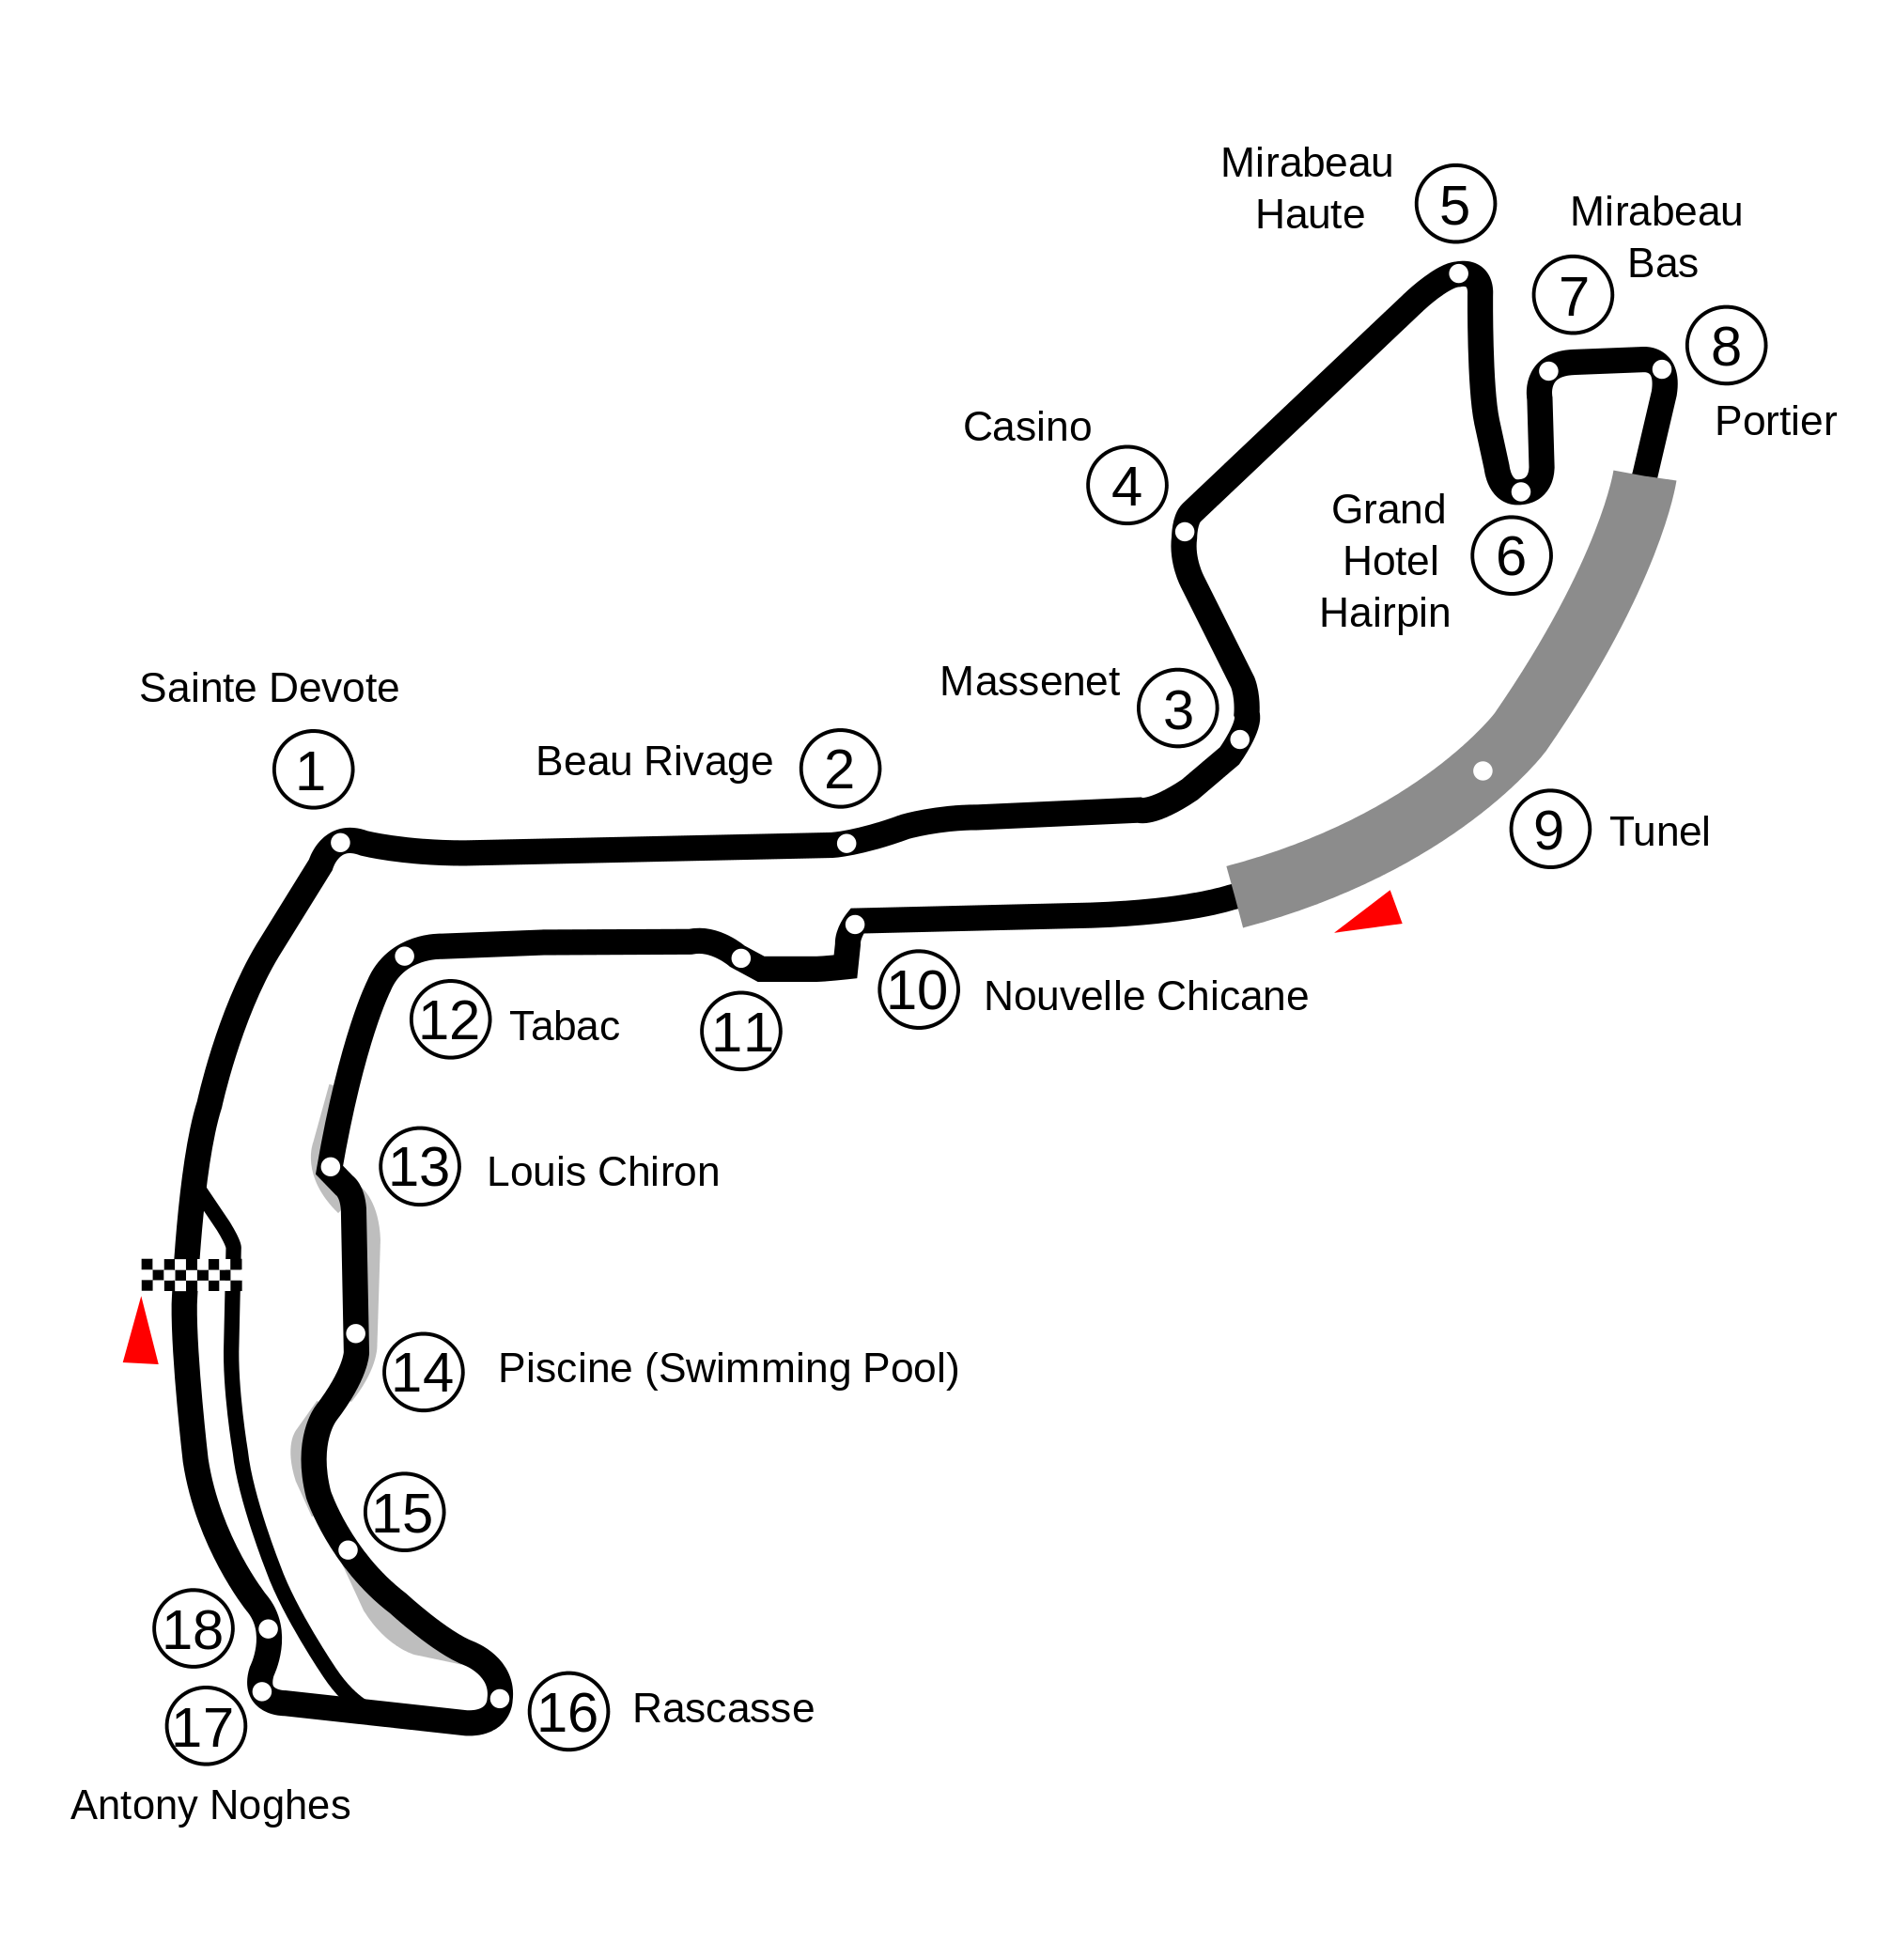
\includegraphics[width=0.5\textwidth]{CircuitoMonaco.png}
	\caption{Trazado del circuito de Mónaco usado como plantilla} \label{fig:circuitomonaco.}
\end{figure}

A continuación añadimos una curva ”Bezier” (\textit{Figura \ref{fig:interfazblender05}}), hacemos esto desde el menú superior en ”Add”, ”Curve”, ”Bezier”. Esto creará un nuevo objeto, que podemos renombrar en la ventana de Objetos para facilitar el acceso y la selección posteriormente, cuando tengamos mas objetos en la escena. Este tipo de curvas, como se puede apreciar en la figura \ref{fig:interfazblender05}, son unas curvas com muchos elementos que nos permiten moldearlas a nuestro gusto. En cada extremo del tramo se componen de una recta con tres puntos. el central que establece el inicio del trazo de la curva, y los otros dos que establecen el giro de la curva y lo pronunciado que és. Cuanto más cerca estén del punto central más cerrado será el ángulo de giro, y cuanto más alejados más suave la curva descrita.

\begin{figure}[h]
	\centering
	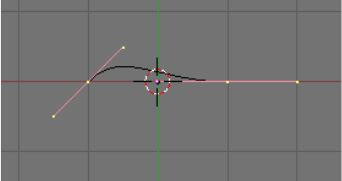
\includegraphics[width=0.3\textwidth]{InterfazBlender05.png}
	\caption{Detalle de curva Bezier.} \label{fig:interfazblender05}
\end{figure}

Al hacer click con el botón izquierdo del ratón mientras mantenemos la tecla Control pulsada añadimos un nuevo punto a la curva ya existente. De esta forma podemos ir añadiendo puntos y deformando la curva hasta que se superponga con la imagen del trazado. Así logramos una curva cerrada correspondiente al trazado sobre la cual situar los elementos que compondrán la carretera, como podemos apreciar en la Figura\ref{fig:monacotrazado} (\textit{La línea naranja es la curva Bezier que será el trazado}).

\begin{figure}[ht]
	\centering
	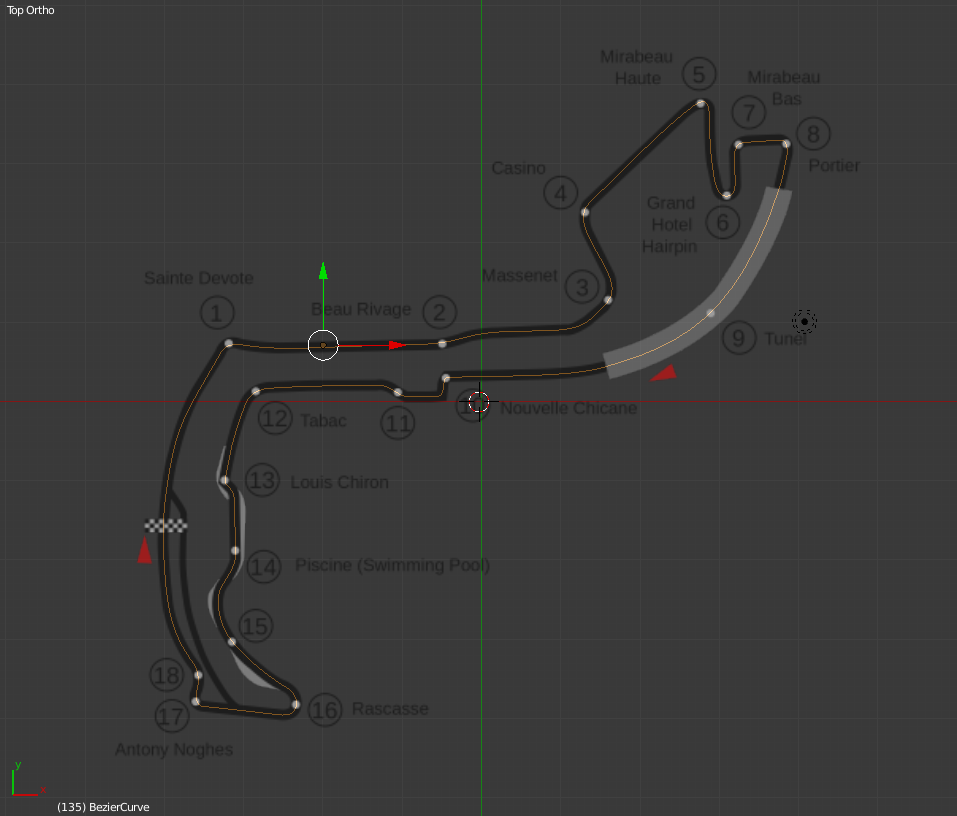
\includegraphics[width=0.6\textwidth]{MonacoTrazado.png}
	\caption{Trazado del circuito de Mónaco superpuesto a la plantilla.} \label{fig:monacotrazado}
\end{figure}

A continuación añadimos un plano haciendo ”Add”, ”Mesh”, ”Plane”, lo cual generará un cuadrado plano en el centro de la escena A continuación seleccionamos una arista u la extruimos (\textit{estiramos}) dos veces, una más corta y una más larga. hacemos lo mismo con la arista opuesta del cuadrado. Es importante realizar este paso ayudándonos de las flechas de colores (\textit{verde, rojo y azul}) que aparecen al seleccionar un objeto para mantener el conjunto en el mismo plano. Una vez realizado, extruimos los dos rectángulos más pequeños hacia arriba, consiguiendo crear la carretera, las vallas y una acera para el circuito, aunque de momento sólo aparecen en gris.

Para ayudarnos en la labor de texturizar objetos, editamos el tipo de ventana que és la de la parte inferior, el gráfico temporal, y lo sustituimos por un Editor de Imagen/UV, el cual posee herramientas avanzadas de manejo de imágenes para texturizado de superficies. De esta manera vamos cara por cara de nuestro objeto seleccionándola en la vista 3D, añadiendo una textura \footnote{Las imágenes usadas como texturas y materiales en este proyecto han sido obtenidas de manera gratuita de la página textures.com\cite{texturescom}} en el Editor UV, y observando los resultados en la vista 3D cambiando el modo de visualización a texturizado. La ventana del Editor de imagen nos sirve para redimensionar las texturas, girarlas, pintar encima de ellas, establecer qué zonas aparecen en la superficie seleccionada, y multitud de herramientas que hacen mucho más sencillo la edición de texturas. Una vez finalizado el paso de texturizar las caras del objeto obtenemos el segmento de la figura \ref{fig:monacosegmento}.

\begin{figure}[h]
	\centering
	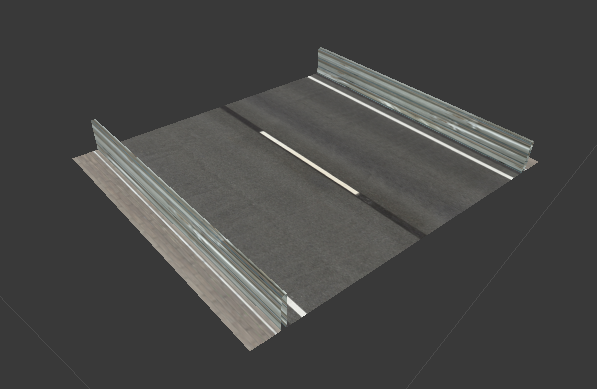
\includegraphics[width=0.4\textwidth]{MonacoSegmento.png}
	\caption{Segmento del circuito.} \label{fig:monacosegmento}
\end{figure}

Es muy importante crear un material para cada textura y asignarlo a las caras correspondientes, de otra manera no se aplicará la textura al renderizar y será como haber trabajado en vano. Esto se consigue mediante la ventana de propiedades y haciendo click en la pestaña de materiales. Es necesario crear un material nuevo, añadir como fuente la misma imagen que se ha usado como textura anteriormente, renombrar para no confundirlos más adelante, y asignarlo a la superficie correspondiente. Además, en la pestaña texturas, debemos repetir los pasos para crear la textura de la misma forma que el material. Necesitaremos además asignar cada textura al material correspondiente y cambiar el tipo de mapping a UV. Es una tarea laboriosa pero muy importante, ya que de no realizarse correctamente las texturas podrían no aplicarse y el objeto aparecería gris.

\begin{figure}[hb]
	\centering
	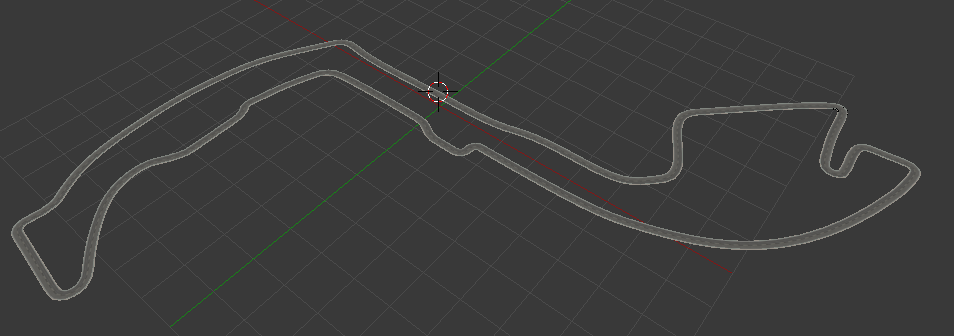
\includegraphics[width=0.8\textwidth]{MonacoTrazado1.png}
	\caption{Circuito (sólo el trazado).} \label{fig:monacotrazado1}
\end{figure}

Una vez realizados todos estos pasos seleccionamos el segmento del trazado creado y vamos a la ventana de propiedades y hacemos click en la pestaña de modificadores. Añadimos un nuevo modificador, un Array. Con esto conseguimos crear multitud de objetos iguales conectados entre sí, como si de un circuito de slot se tratase. Despues añadimos otro modificador, una curva en este caso, y elegimos como elemento modificante la curva Bezier que hemos creado anteriormente. De esta manera, jugando con el número de copias que realiza el array, conseguimos que el segmento creado se repita y deforme siguiendo el trazado de la curva, adquiriendo la forma del circuito deseado. Este método requiere de muchos retoques manuales, ya que en los vértices de las curvas cerradas el programa no puede calcular bien y solapa y deforma de manera incorrecta los vértices del segmento. Una vez realizados todos los retoques, así como la unión del primer y último segmento, obtenemos el objeto de la figura \ref{fig:monacotrazado1}.

Una vez obtenido el trazado necesitamos añadir un plano que serfirá de fondo para el circuito. Para ello añadimos un nuevo objeto plano a la escena, lo aumentamos de tamaño hasta que se pueda situar el circuito en su interior y lo subdividimos en cuadrículas. Esto lo hacemos así para poder asignar texturas a cada cuadrícula independientemente y simular de manera más realista que este circuito se sitúa en un puerto, estando a la orilla del mar casi la mitad de su recorrido. Una vez realizada la división deformamos algunos vértices escondiéndolos debajo del trazado, necesitando así menos divisiones y aligerando la carga de procesamiento del circuito. Una vez asignadas todas las texturas, repitiendo los pasos descritos para texturizar el segmento del circuito, obtenemos el circuito de Mónaco\ref{fig:monacoplano1}, el cual podemos ver en detalle en la Figura \ref{fig:monacoplanovistas}.

\begin{figure}[t]
	\centering
	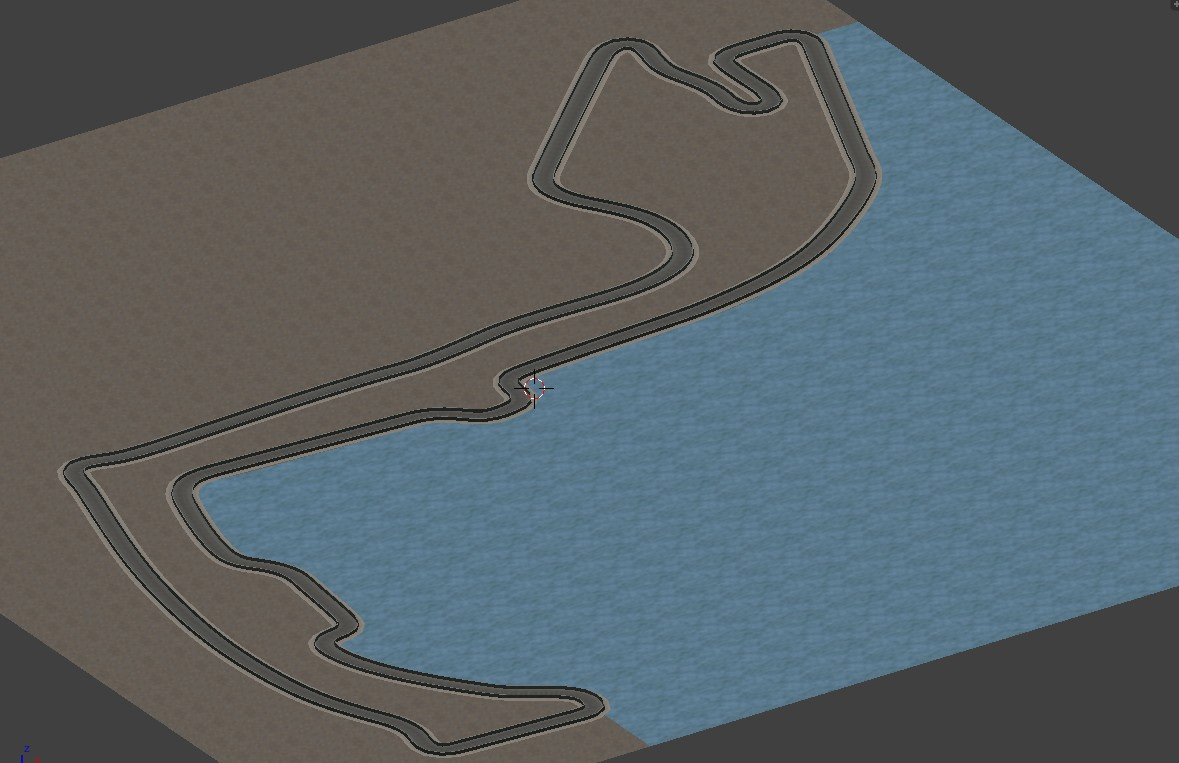
\includegraphics[width=0.7\textwidth]{MonacoPlano1.jpg}
	\caption{Circuito plano.} \label{fig:monacoplano1}
\end{figure}

\begin{figure}
	\centering
	\subfigure{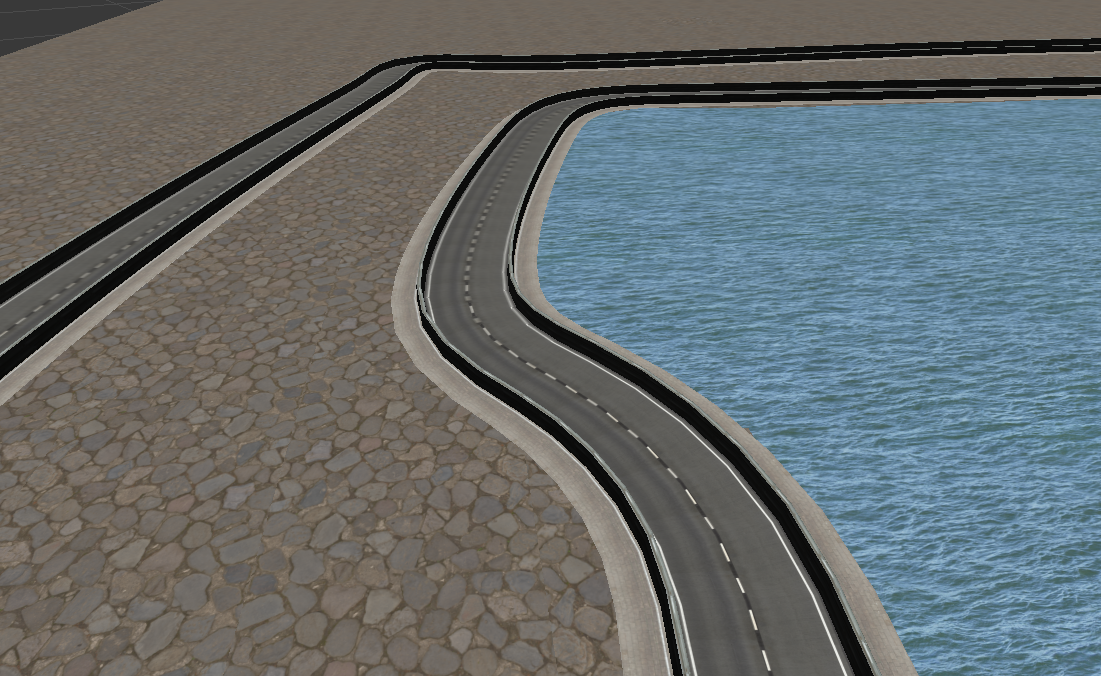
\includegraphics[width=0.4\textwidth]{MonacoPlano2.png}}\hspace{0.04\textwidth}	
	\subfigure{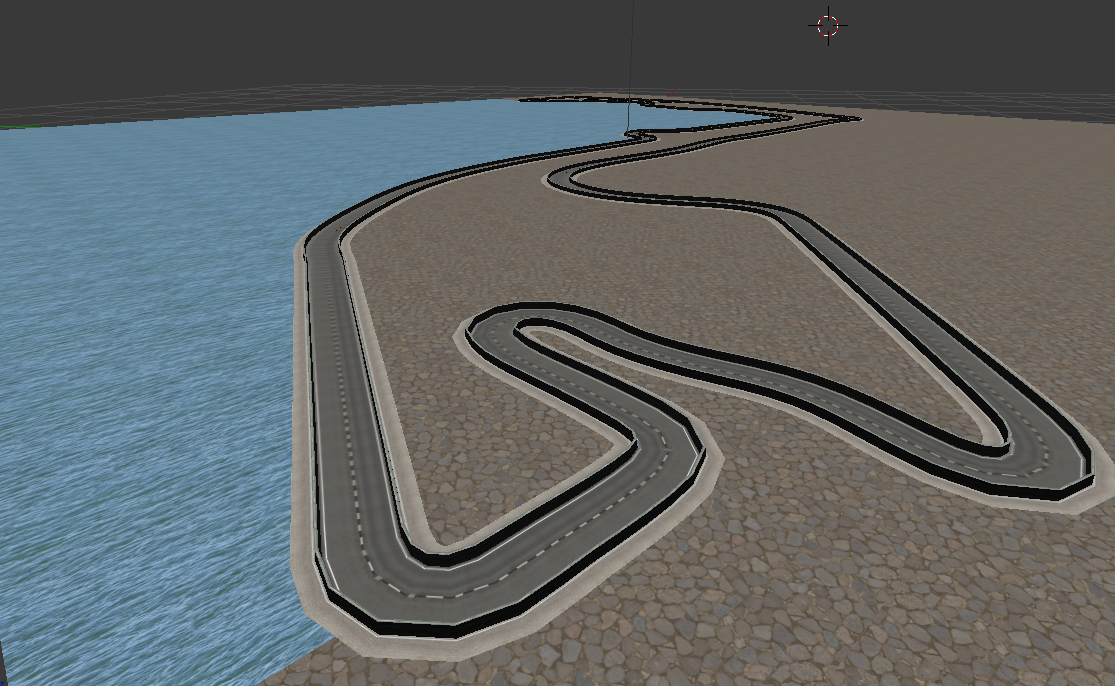
\includegraphics[width=0.4\textwidth]{MonacoPlano9.png}}\vspace{0.03\textwidth}
	\subfigure{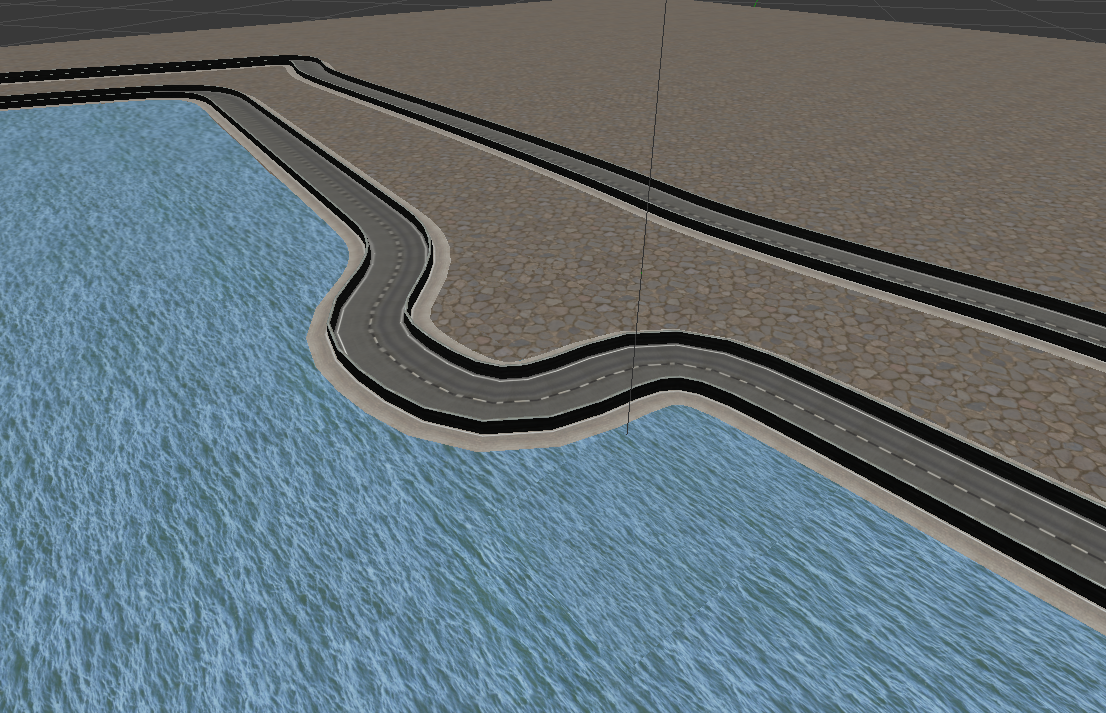
\includegraphics[width=0.4\textwidth]{MonacoPlano10.png}}\hspace{0.04\textwidth}
	\subfigure{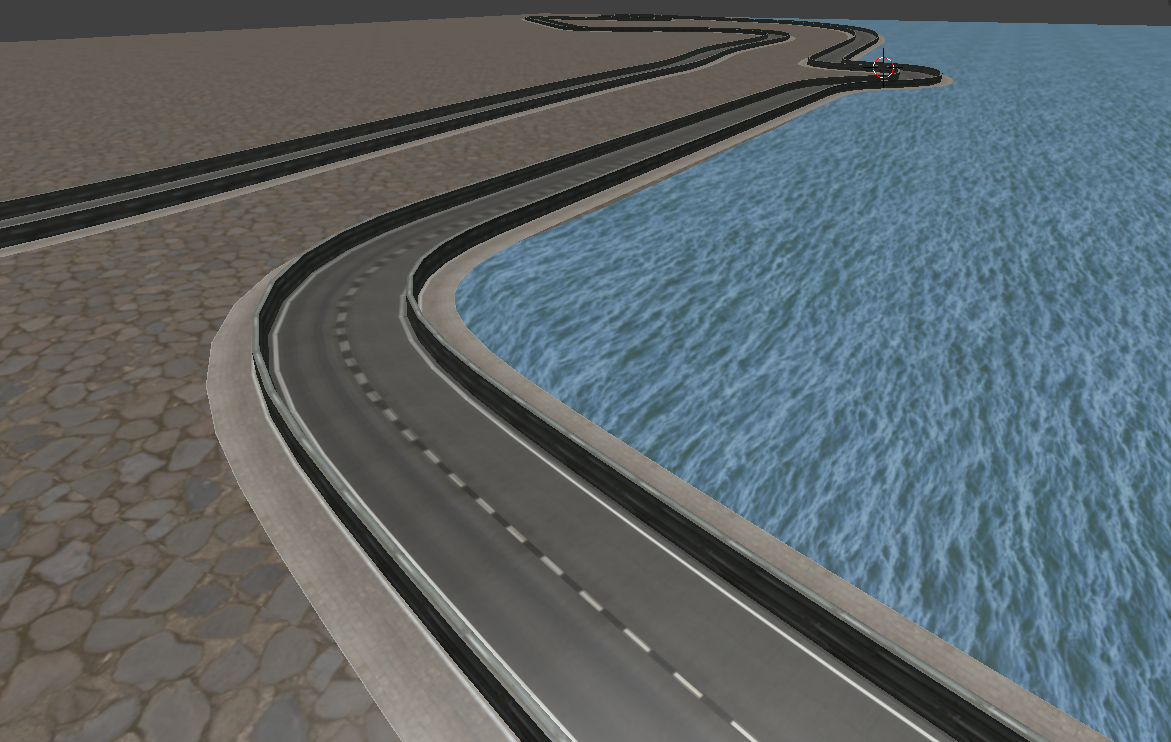
\includegraphics[width=0.4\textwidth]{MonacoPlano3.png}}
	\caption{Diferentes vistas del circuito de F1 de Mónaco plano} \label{fig:monacoplanovistas}
\end{figure}


\section{Circuito con elevaciones}
\label{sec:pm_circuitoconelevaciones}

Una vez modelado el circuito plano pasamos a modelarlo ahora con elevaciones. Dada la dificultad de simplemente añadirlas al circuito ya creado, partimos de cero en la creación de este nuevo escenario. Puesto que ahora es mucho más relevante el fondo comenzamos por esa parte. Eliminamos el cubo por defecto y añadimos un nuevo objeto, ésta vez una ”Mesh”, ”Grid”, que llamaremos rejilla. Es diferente del plano por que ya está subdividido, como una rejilla. Al crearlo, en la parte inferior izquierda de la ventana de vista 3D, aparecen una serie de propiedades únicas de este objeto que modificamos a nuestro gusto, en este caso el numero de subdivisiones de la rejilla y el tamaño de ésta.

Haciendo click en el botón de Modo Edición accedemos a otro modo, en este caso de Escultura. Una vez en este modo, en la parte superior izquierda de la ventana de vista 3D se despliega una multitud de herramientas y opciones para esculpir los objetos de la escena. Como lo que nos interesa es elevar la rejilla de forma que simule las alturas y elevaciones del circuito real de Mónaco, accedemos a la opción de bloqueo y seleccionamos los ejes x e y, con lo que sólo modificaremos la altura del plano sobre el que proyectaremos el trazado. Modificando las opciones del pincel hasta dejarlo a nuestro gusto comenzamos a esculpir la rejilla. Usando la misma imagen de antes como plantilla de fondo y fotos reales del circuito esculpimos un prototipo de lo que serán las elevaciones, que más tarde retocaremos para ajustarnos mejor a las peculiaridades del trazado. También nos serviremos de otro tipo de pincel para alisar las rugosidades creadas al modelar de forma mas basta y así suavizar el terreno para acomodar mejor al circuito.

\begin{figure}[t]
	\centering
	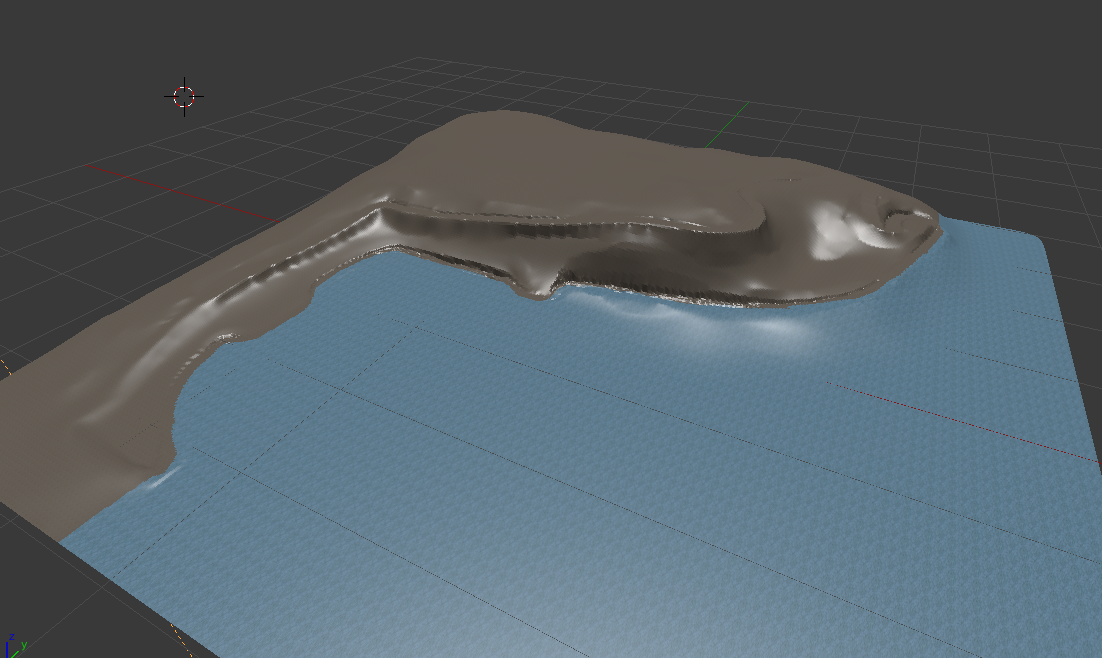
\includegraphics[width=0.7\textwidth]{MonacoElev00.png}
	\caption{Fondo para el circuito con elevaciones.} \label{fig:monacoelev00}
\end{figure}

A continuación creamos de nuevo, siguiendo los mismos pasos, la curva Bezier que servirá de trazado. Creamos ahora un plano, que pintamos de un color llamativo, y extendemos a lo largo de la curva bezier, consiguiendo un trazado de referencia para acabar de dar los últimos detalles a la rejilla. Tanto a la curva como a este plano le aplicamos como modificador la rejilla, consiguiendo darles altura y pudiendo ver el recorrido real del circuito con las elevaciones modeladas. Ahora modelamos la rejilla teniendo en cuenta el recorrido del circuito y su situación a orillas del mar, por lo que tenemos mucho cuidado de mantener plana toda la parte baja y del mar y aplicamos las elevaciones en las demás partes. Una vez modelado texturizamos de forma análoga a como hicimos anteriormente. Una vez modelado y texturizado el plano, eliminamos el trazado de referencia y obtenemos el suelo sobre el que descansará el circuito (\textit{Figura \ref{fig:monacoelev00}}).

\begin{figure}[hb]
	\centering
	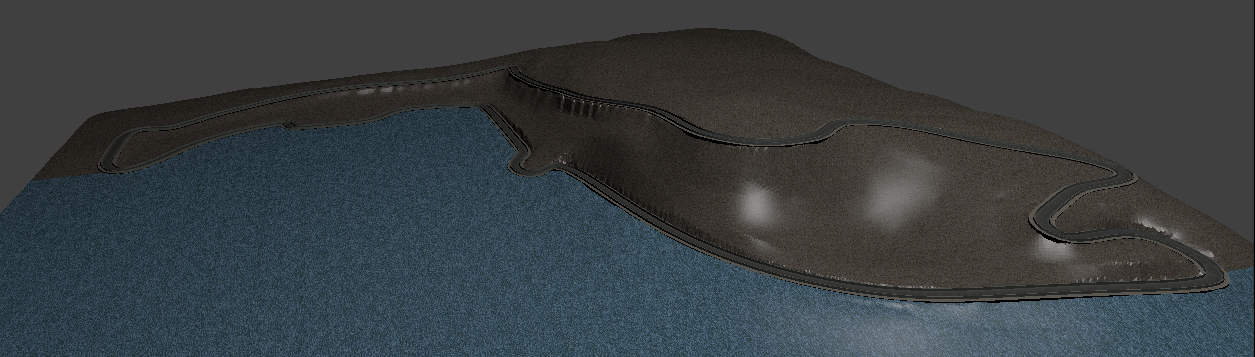
\includegraphics[width=0.9\textwidth]{MonacoElev05.png}
	\caption{Circuito con elevaciones.} \label{fig:monacoelev05}
\end{figure}

Ahora repetiremos todos los pasos de creación del trazado (creamos el segmento, lo texturizamos, lo extendemos a lo largo de la curva) y además le aplicamos la rejilla como modificador. Si hemos realizado bien el paso anterior con el trazado de referencia, el trazado final debería descansar sobre la caja realizada y acoplarse perfectamente al terreno, de no ser así retocamos nuevamente la rejilla con las herramientas de escultura. 

Una vez completado este paso podemos dar por finalizado el circuito (\textit{Figura \ref{fig:monacoelev05}}). En la Figura \ref{fig:monacoelevvistas} se pueden ver detalles del circuito donde se aprecian mejor las elevaciones del terreno.

\begin{figure}[h]
	\centering
	\subfigure{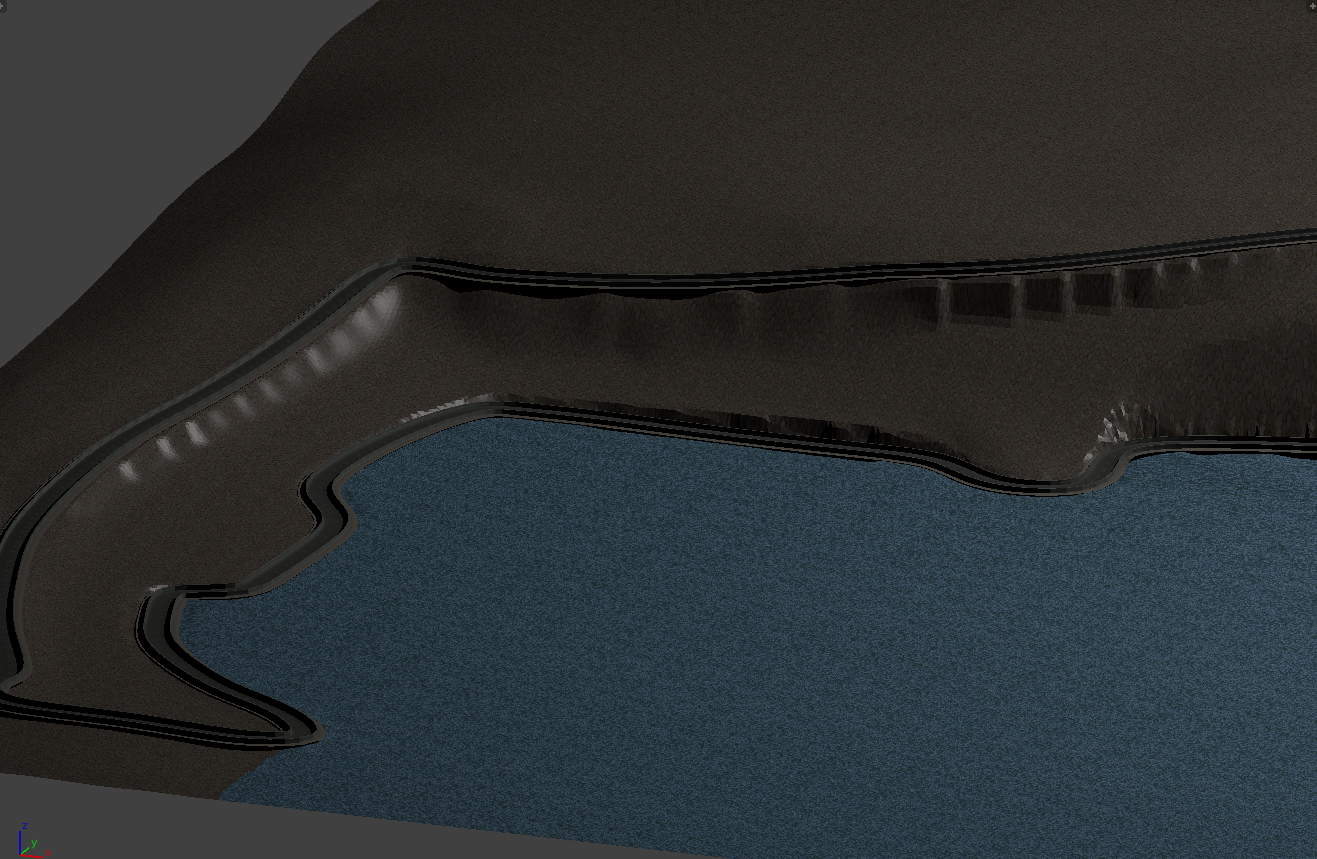
\includegraphics[width=0.4\textwidth]{MonacoElev01.png}}\hspace{0.04\textwidth}	
	\subfigure{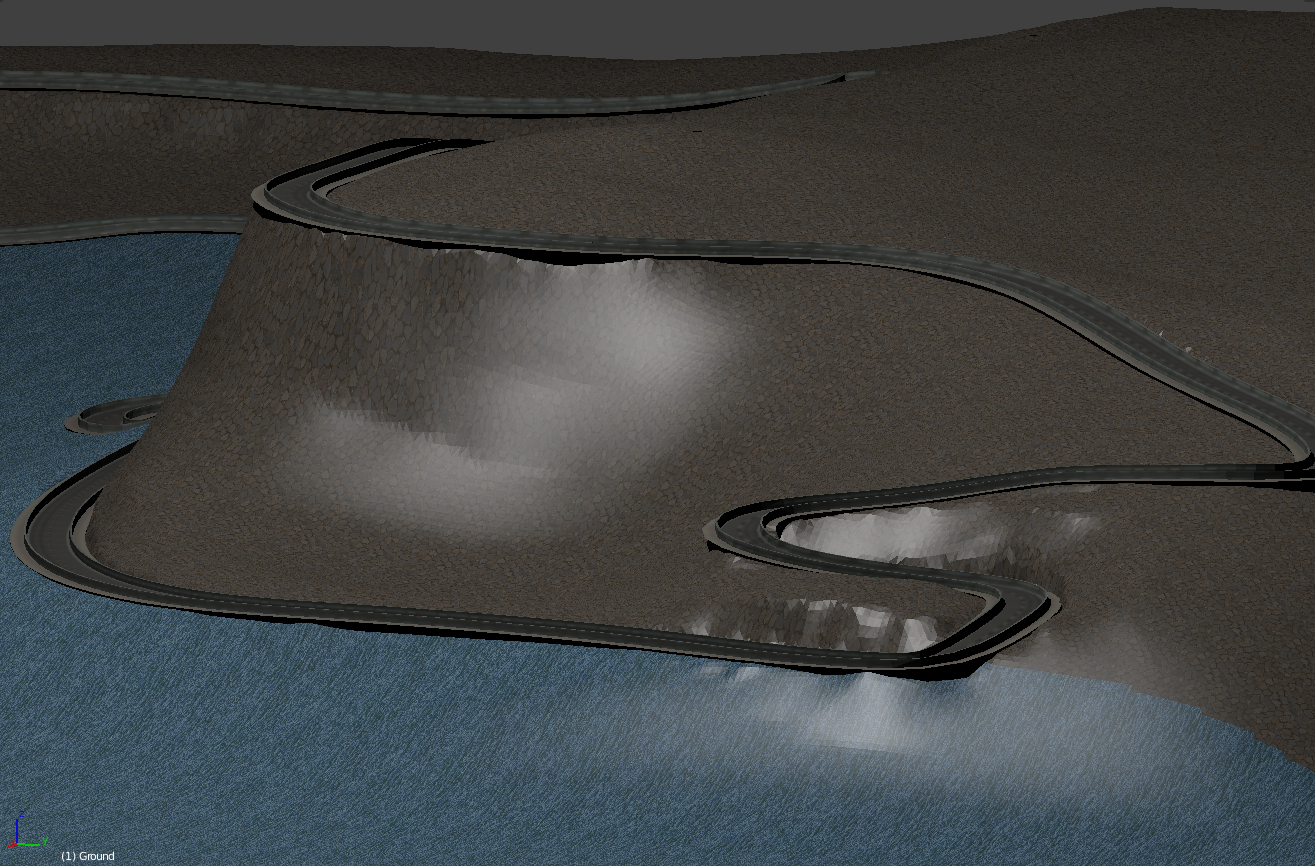
\includegraphics[width=0.4\textwidth]{MonacoElev02.png}}\vspace{0.03\textwidth}
	\subfigure{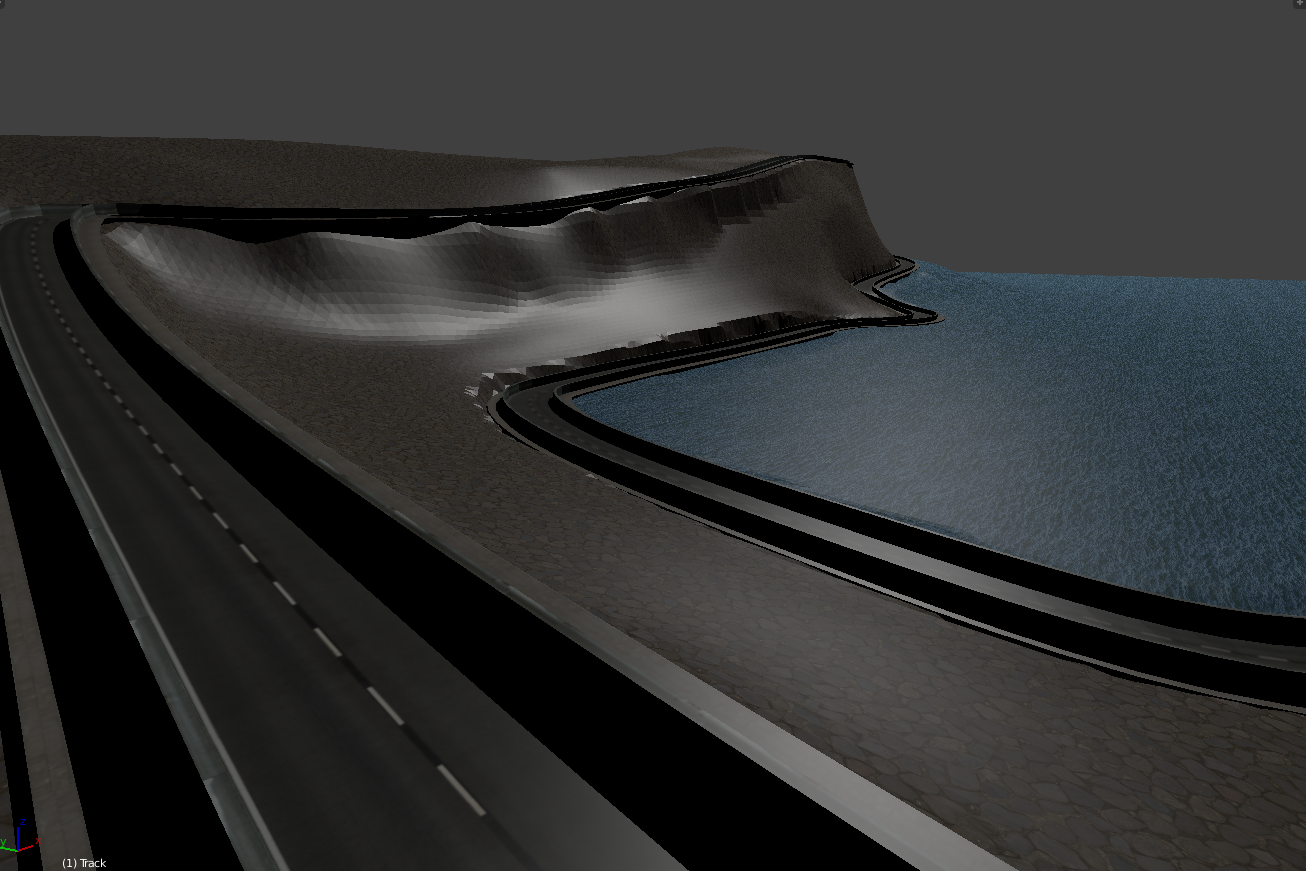
\includegraphics[width=0.4\textwidth]{MonacoElev03.png}}\hspace{0.04\textwidth}
	\subfigure{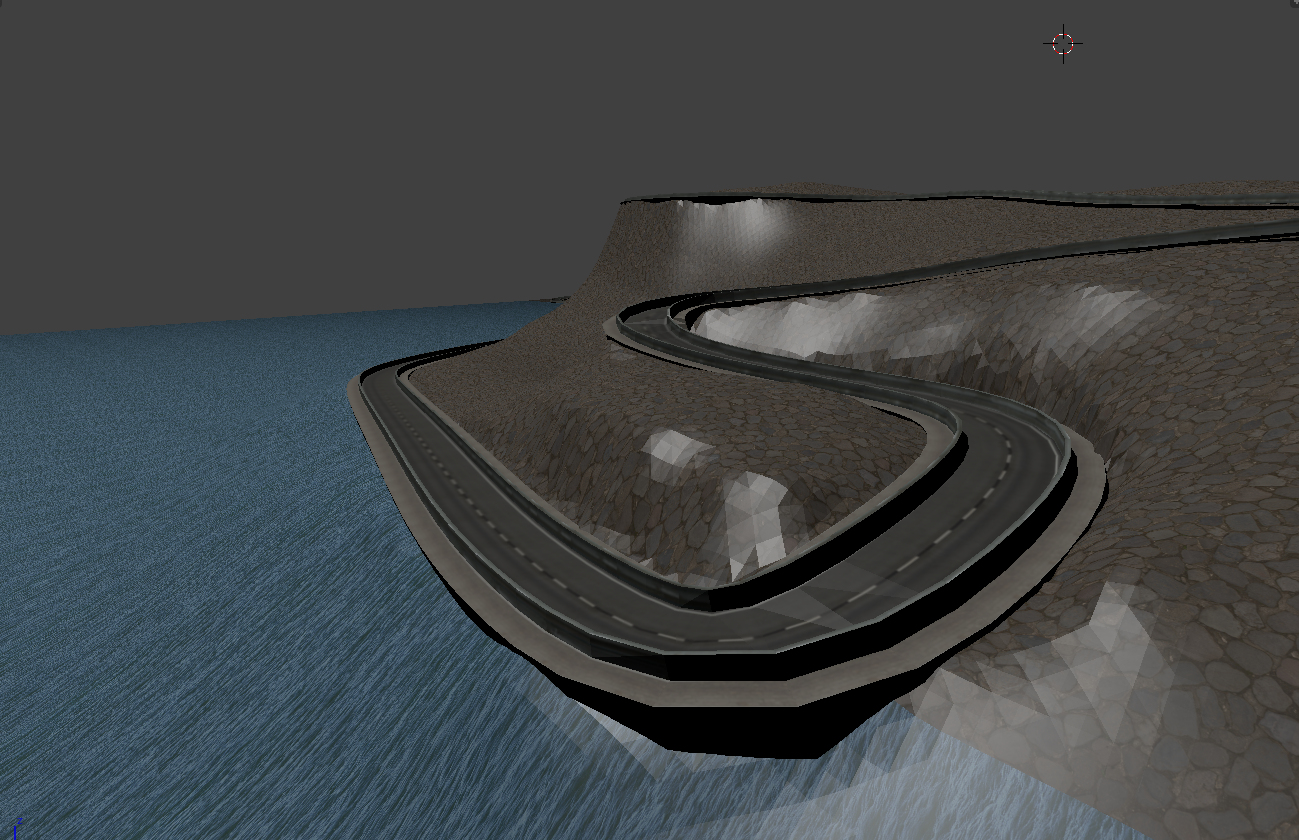
\includegraphics[width=0.4\textwidth]{MonacoElev04.png}}
	\caption{Diferentes vistas del circuito de F1 de Mónaco con elevaciones} \label{fig:monacoelevvistas}
\end{figure}



\section{Mundos para Gazebo}
\label{sec:pm_mundosparagazebo}




